\documentclass[12pt]{article}
\usepackage{graphicx}
\begin{document}
{\bf Names:} Jack Bracewell, Milan Misak, Craig Ellis \\
{\bf Usernames:} jb2910, mm5510, ce710 \\
{\bf Group Number: 28}  \\ \\

{\bf Assignment 2:} Decision Trees Algorithm \\ \\

{\bf Implementation details} \\
\begin{itemize}
  \item Cross-validation was done by first generating a cell array of the binary targets for each emotion. Then, inside a for-loop, each fold is removed from the set of examples in turn, leaving a set used to train the decision tree, and the fold used to test the resulting trees for accuracy. A running total is kept of correct answers, along with a confusion matrix updated on each loop.
  \item Best attributes were selected in the suggested manner, by keeping track of p$_{\textrm{0}}$, n$_{\textrm{0}}$, p$_{\textrm{1}}$, and n$_{\textrm{1}}$ in the loop for each attribute, and using the provided formulae to compute whether or not the new attribute provides a greater information gain than the previous best.
  \item All data for the average cross-validation results is collected during the cross-validation, with a running total of correct answers, and the incrementation of entries in the confusion matrix. A call is made to a seperate function to get recall and precision rates, as well as F$_{\textrm{1}}$ measures, to keep the code tidier.
\end{itemize}

{\bf Generated trees} \\ \\
\begin{center}
  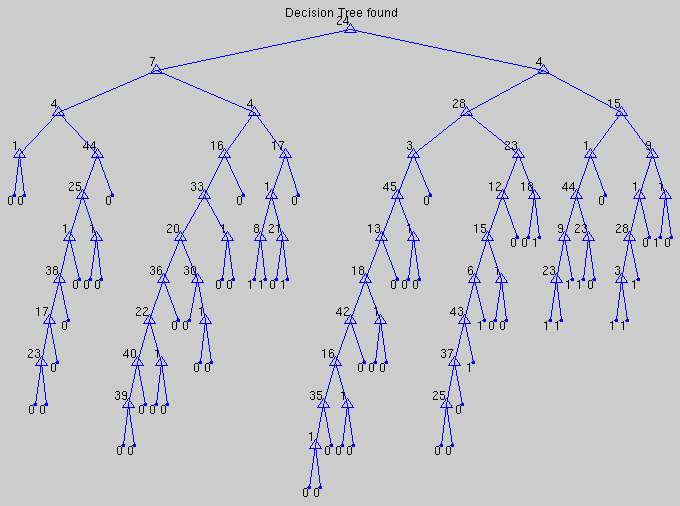
\includegraphics[scale=0.28]{report-images/tree1.png} \\
  Tree for emotion 1 \\
  \vspace{\baselineskip}
  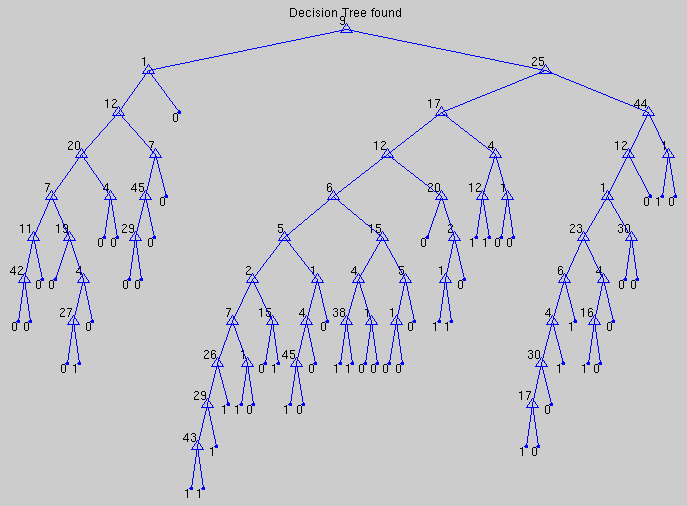
\includegraphics[scale=0.28]{report-images/tree2.png} \\
  Tree for emotion 2 \\
  \vspace{\baselineskip}
  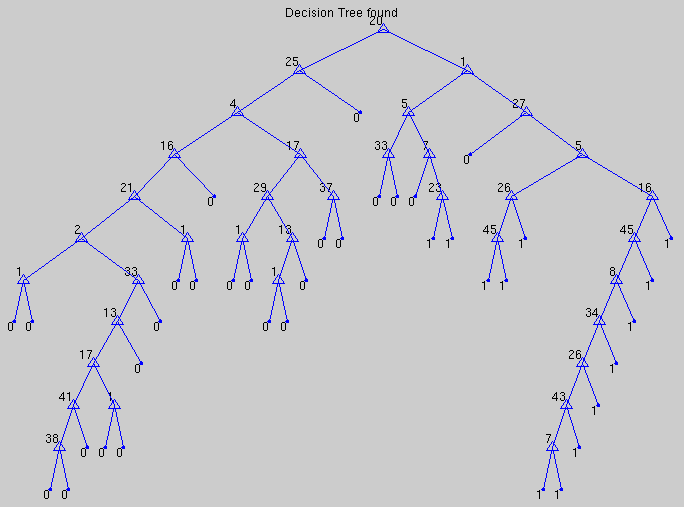
\includegraphics[scale=0.28]{report-images/tree3.png} \\
  Tree for emotion 3 \\
  \vspace{\baselineskip}
  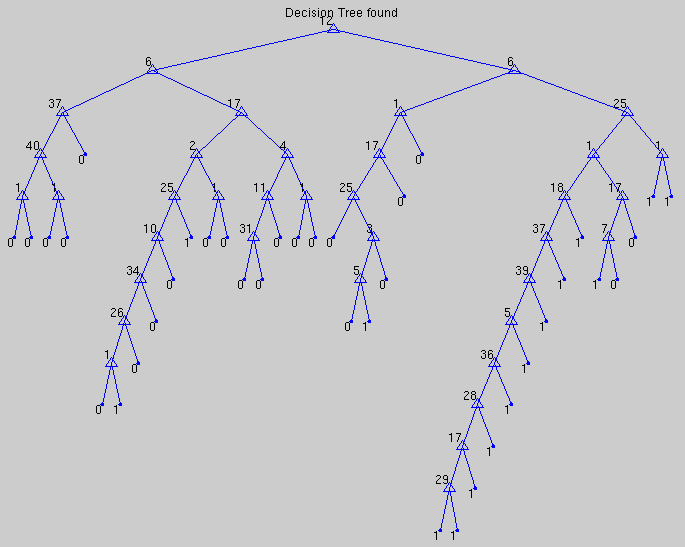
\includegraphics[scale=0.28]{report-images/tree4.png} \\
  Tree for emotion 4 \\
  \vspace{\baselineskip}
  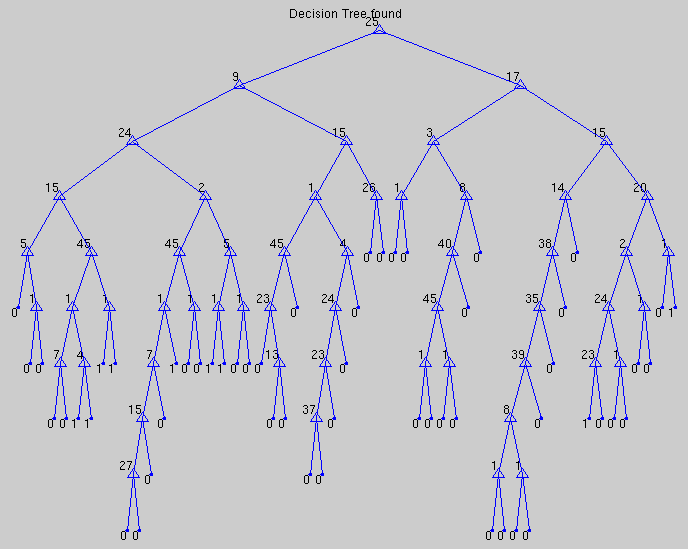
\includegraphics[scale=0.28]{report-images/tree5.png} \\
  Tree for emotion 5 \\
  \vspace{\baselineskip}
  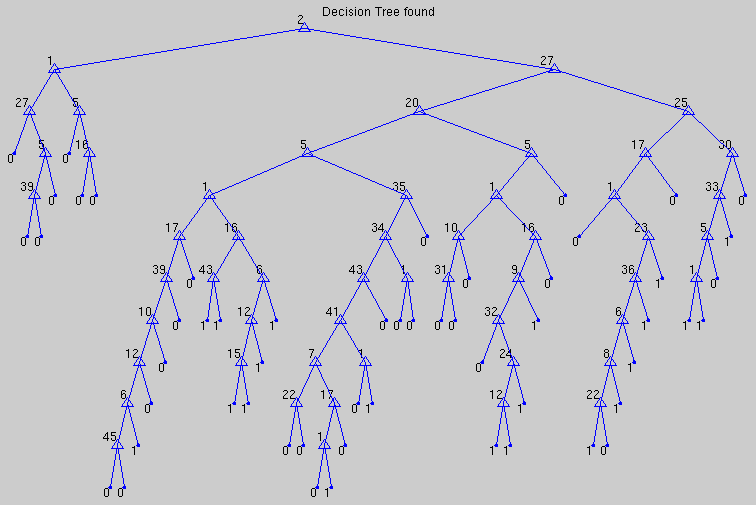
\includegraphics[scale=0.28]{report-images/tree6.png} \\
  Tree for emotion 6 \\
  \vspace{\baselineskip}
\end{center}

{\bf Evaluation results} \\
Confusion matrix, av. classification rate, av. precision/recall rates, F-measure; include comments \\ \\

{\bf Ambiguity} \\
Answer sheet question \\ \\

{\bf Pruning} \\
Answer sheet question\\ \\

{\bf Code Flowchart} \\
Flowchart of code workings\\ \\

\end{document}
